\chapter{Transformation Techniques}\indexmain{imperativeandstate}
\label{cha:techniques}
\label{sub:mergesplit}

In this chapter we'll have a look at transformation techniques to solve common graph rewriting tasks utilizing the constructs introduces so far.
They could be offered directly by some dedicated operators,
but these would need so much customization to be useful in the different situations one needs them,
that we decided against dedicated operators;
instead it is on you to program the version you need yourself by \emph{combining} language constructs and rules.

The primary means to build transformations are top-level \emph{sequences}, controlling rule applications (on one or all matches).
They may call other sequences, even so recursively.
The sequences allow for \emph{external composition} of rules; a rule may be \emph{(re-)used} multiple times.
They follow the \emph{imperative} programming paradigm, one rule is applied after the other, on the \emph{then-changed} state (of the graph, changed after each step).

With \emph{embedded sequences} are you able to call rules from within a rule application, after the rule proper was executed (deferred execution), with direct access to the elements of that rule.
Seen from the outside, they allow to build a complex rule and thus allow for rule \emph{internal composition}, again in an \emph{imperative} way.
They allow to do work later on you can't do while executing the rule proper (e.g. because an element was already matched and is now locked due to the isomorphy constraint), to follow a breadth-splitting structure, or simply to split work into several parts, modularizing it, \emph{reusing} already available functionality.

The other means for \emph{internal composition} are the \emph{nested and subpatterns}.
They allow to match and rewrite complex patterns built in a structured way piece by piece.
With different pieces connected together, pieces to decide in between, and pieces which appear repeatedly.
They follow the \emph{functional} programming paradigm, a complex state change is built compositionally without graph changes in between, only after applying the rule in a big step is the graph changed (in fact after the rewriting half-step, following the matching half-step). 
They shift processing below the rules-combined-by-sequences level. 

The sequences typically use graph-element-valued variables to communicate a \emph{single spot} in the host graph that is currently getting processed in between the rules.
This can be generalized with \emph{storages (container variables)} capable of holding \emph{multiple spots}; they allow to store elements collected in one run and reuse them as input in another run (this is esp. useful if elements are reached on different paths).
You can break up a transformation into self-contained \emph{passes} mediated by some \emph{intermediate state} with those multi-valued variables. 

Besides, you can employ elementary procedures directly manipulating the graph and elementary functions directly querying the graph, combining them \emph{programmatically} with expressions and statements, abstracting them into own procedures and functions.
Those functions and procedures can then be \emph{used} from the \texttt{if} and \texttt{eval} parts of the rules, and from the sequences.

\begin{note}
Prefer declarative composition, it helps in keeping the code readable and easily adaptable.
Prefer internal embedding over external state passing, it is typically a good deal more concise.
But don't go to extremes regarding this, use the mode of composition that is suited to the task and feels best and most natural.

Avoid rules carrying out a tiny amount of work with a lot of input and output and heavy external orchestration (graph-rewriting,  assembler-level style), aim for a medium amount of work per rule call (well, normally more is better, but when you press too hard you can get over the top).
\end{note}

\begin{note}
An alternative to storage containment are visited flags, they allow to mark interesting elements directly.
The storage sets are more efficient compared to the visited flags in case the count of elements of interest is a good deal smaller than the number elements in the graph; they are looked up in the set, in contrast to the visited flags, which are used by enumerating all available graph elements, filtering according to the visited state.
The visited flags on the other hand are extremely memory efficient (for free as long as you use only a few of them at the same time).
\end{note}

\begin{note}
Don't forget the last resort if you must solve a task so complex that the above means of composition (regarding control-flow or data-flow) are not sufficient: adding helper nodes, edges, or attributes to the graph model and the graph itself, holding some intermediate state of processing. 
\end{note}

In the following we'll employ those constructs to merge and split nodes, emulate node replacement grammars, execute transformations in the narrow sense, aka mappings, copy substructures, compute flow equations over the graph structure with sets in the nodes, and enumerate state spaces.
Further examples can be found in \cite{CompilerOptimization} employing two storagesets switched in between for computing a wavefront running over a compiler graph and \cite{ProgramUnderstanding} using the nested and subpatterns for elegantly extracting a state machine model from a program graph.


\section{Merge and Split Nodes}\indexmain{merge node}\indexmain{split node}
Merging a node \texttt{m} into a node \texttt{n} means transferring all edges from node \texttt{m} to node \texttt{n}, then deleting node \texttt{m}.
Splitting a node \texttt{m} off from a node \texttt{n} means creating a node \texttt{m} and transferring some edges from node \texttt{n} to \texttt{m}.

In both cases there are a lot of different ways how to handle the operation exactly:
Maybe only incoming or only outgoing edges, or only edges of a certain type \texttt{T} or only edges not of type \texttt{T}; maybe the node \texttt{n} is to be retyped, maybe the edges are to be retyped.
But common is the transferring of edges; this can be handled succinctly by an \texttt{iterated} statement and the \texttt{copy} operator.
In case the node opposite to an edge may be incident to several such edges, one must use an \texttt{exec} instead (or the \texttt{independent} operator \ref{rule:homspec}), as every iteration locks the matched entities, so they can't get matched twice. Not needing the opposite node one could simply leave it unmentioned in the pattern, only referencing node \texttt{n} or \texttt{m} and the edge, but unfortunately we need the opposite node so we can connect the edge copy to it.

\begin{note}
In case a simple node merging without edge retyping is sufficient the retype'n'merge clause introduced in \ref{sec:merge} offers a much simpler alternative for merging.
\end{note}

Now we'll have a look at an example for node merging: T1-T2 analysis from compiler construction is used to find out whether a control flow graph of a subroutine is reducible, i.e. all loops are natural loops. All loops being natural loops is a very useful property for many analyses and optimizations. The analysis is split into two steps, T1 removes reflexive edges, T2 merges a control flow successor into its predecessor iff there is only one predecessor available. These two steps are iterated until the entire graph is collapsed into one node which means the control flow is reducible, or execution gets stuck before, in which case the control flow graph is irreducible.

The analysis is defined on simple graphs, i.e. if two control flow edges between two basic block nodes appear because of merging they are seen as one, i.e. they are automatically fused into one. As \GrG~is built on multigraphs we have to explicitly do the edge fusion in a further step T3.

First let us have a look at T1 and T3, which are rather boring ... ehm, straight forward:

  \begin{example}
    \begin{grgen}
rule T1 {
  n:BB -:cf-> n;

  replace {
    n; // delete relexive edges
  }
}
rule T3 {
  pred:BB -first:cf-> succ:BB;
  pred    -other:cf-> succ;

  modify { // kill multiedges
    delete(other);
  }
}
    \end{grgen}
  \end{example}

The interesting part is T2, this is the first version using an iterated statement:

  \begin{example}
    \begin{grgen}
rule T2 {
  pred:BB -e:cf-> succ:BB;
  negative {
    -e->;
    -:cf-> succ; // if succ has only one predecessor
  }
  iterated {
    succ -ee:cf-> n:BB;

    modify { // then merge succ into this predecessor
      pred -:copy<ee>-> n; // copying the succ edges to pred
    }
  }

  modify { // then merge succ into this predecessor
    delete(succ);
  }
}
    \end{grgen}
  \end{example}

In case a control flow graph would be a multi-graph, with several control flow edges between two nodes, one would have to use an \texttt{exec} with an all-bracketed rule instead of the \texttt{iterated}, to be able to match a multi-\texttt{cf}-edge target of \texttt{succ} multiple times (which is prevented in the \texttt{iterated} version by the isomorphy constraint locking the target after the first match).

This is the second version using exec instead, capable of handling multi edges:

  \begin{example}
    \begin{grgen}
rule T2exec
{
  pred:BB -e:cf-> succ:BB;
  negative {
    -e->;
    -:cf-> succ; // if succ has only one predecessor
  }

  modify { // then merge succ into this predecessor
    exec([copyToPred(pred, succ)] ;> delSucc(succ));
  }
}

rule copyToPred(pred:BB, succ:BB)
{
  succ -e:cf-> n:BB;

  modify {
    pred -:copy<e>-> n;
  }
}

rule delSucc(succ:BB)
{
  modify {
    delete(succ);
  }
}
    \end{grgen}
  \end{example}

Natural loops are so advantageous that one transforms irreducible graphs (which only occur by using wild gotos) into reducible ones, instead of bothering with them in the analyses and optimizations.
An irreducible graph can be made reducible by node splitting, which amounts to code duplication (in the program behind the control flow graph).
In a stuck situation after T1-T2 analysis, a \texttt{BB} node with multiple control flow predecessors is split into as many nodes as there are control flow predecessors, every one having the same control flow successors as the original node.
(Choosing the \texttt{cf} edges and \texttt{BB} nodes which yield the smallest amount of code duplication is another problem which we happily ignore here.)

  \begin{example}
We do the splitting by keeping the indeterministically chosen first cf edge, splitting off only further cf edges, replicating their common target.

    \begin{grgen}
rule split(succ:BB)
{
  pred:BB -first:cf-> succ;
  multiple {
    otherpred:BB -other:cf-> succ;

    modify {
      otherpred -newe:cf-> newsucc:copy<succ>;
      delete(other);
      exec(copyCfSuccFromTo(succ, newsucc));
    }
  }

  modify {
  }
}

rule copyCfSuccFromTo(pred:BB, newpred:BB)
{
  iterated {
    pred -e:cf-> succ:BB;

    modify {
      newpred -:copy<e>-> succ;
    }
  }

  modify {
  }
}
    \end{grgen}
  \end{example}

The examples given can be found in the \texttt{tests/mergeSplit/} directory including the control scripts and test graphs; you may add \texttt{debug} prefixes to the \texttt{exec} or \texttt{xgrs} statements in the graph rewrite script files and call GrShell with e.g. \texttt{mergeSplit/split.grs} as argument from the \texttt{tests} directory to watch execution.


\section{Node Replacement Grammars}\indexmain{node replacement grammar}\indexmainsee{edNCE}{node replacement grammar}
With node replacement grammars we mean edNCE grammars \cite{NodeReplacement}, which stands for edge label directed node controlled embedding. In this context free graph grammar formalism, every rule describes how a node with a nonterminal type is replaced by a subgraph containing terminal and nonterminal nodes and terminal edges. The nodes in the instantiated graph get connected to the nodes that were adjacent to the initial nonterminal node, by connection instructions which tell which edges of what direction and what type are to be created for which original edges of what direction and what type, going to a node of what type.

This kind of grammars can be encoded in \GrG~by rules with a left hand side consisting of a node with a type denoting a nonterminal and iterateds matching the edges and opposite nodes it is connected to of interest; "of interest" amounts to the type and direction of the edges and the type of the opposite node. The right hand side deletes the original node (thus implicitly the incident edges), creates the replacement subgraph, and tells in the rewrite part of the iterateds what new edges of what directedness and type are to be created, from the newly created nodes to the nodes adjacent to the original node. (Multiple edges between two nodes are not allowed in the node replacement formalism, in case you want to handle them you've to use \texttt{exec} as shown in the merge/split example above.)

The following example directly follows this encoding:

  \begin{example}
This is an example rule replacing a nonterminal node \texttt{n:NT} by a 3-clique.
For the outgoing \texttt{E1} edges of the original node, the new node \texttt{x} receives incoming \texttt{E2} edges.
And for incoming \texttt{E2} edges of the original node, the new nodes \texttt{y} and \texttt{z} receive edges of the same type, \texttt{y} with reversed direction and \texttt{z} of the exact dynamic subtype bearing the same values as the original edges.
    \begin{grgen}
rule example
{
  n:NT;

  iterated {
    n -:E1-> m:T;

    modify {
      x <-:E2- m;
    }
  }

  iterated {
    n <-e2:E2- m:T;

    modify {
      y -:E2-> m;
      z <-:copy<e2>- m;
    }
  }

  modify {
    delete(n);
    x:T -- y:T -- z:T -- x;
  }
}
    \end{grgen}
  \end{example}

As another example for node replacement grammars we encode the two rules needed for the generation of the completely connected graphs (cliques) in two \GrG~rules. The first replaces the nonterminal node by a new nonterminal node linked to a new terminal node, connecting both new nodes to all the nodes the original nonterminal node was adjacent to. The second replaces the nonterminal node by a terminal node, connecting the new terminal node to all the nodes the original nonterminal node was adjacent to. This "we want to preserve the original edges" can be handled more succinctly and efficiently by retyping which we gladly use instead of the iteration.

  \begin{example}
    \begin{grgen}
rule cliqueStep
{
  nt:NT;

  iterated {
    nt -- neighbour:T;

    modify {
      t -- neighbour;
      nnt -- neighbour;
    }
  }

  modify {
    delete(nt);
    t:T -- nnt:NT;
  }
}

rule cliqueTerminal
{
  nt:NT;

  modify {
    :T<nt>;
  }
}
    \end{grgen}
  \end{example}

The examples can be found in the \texttt{tests/nodeReplacementGrammar} directory.


\section{Mapping in a Rewriting Tool}\label{sec:transfo}\indexmain{transformation in a narrow sense}
\GrG{} is a \emph{rewrite} tool, i.e. you modify \emph{one} graph.
This is in contrast to \emph{transformation} or better \emph{mapping} tools, which are used for specifying mappings in between \emph{two} (or more) graphs. (Graphs are typically called models in this kind of tools. Don't confuse this with the notion of graph model in \GrG\ as introduced in chapter \ref{chapmodellang}. In model transformation parlance our graph model denotes a meta model, with a model adhering to a meta model, which in turn adheres to a meta meta model, climbing a ladder of bullshit abstraction leading right into the land of the hot-air merchants, eh..., the truthfully real software engineers. XML. Model. Meta. Meta-meta. Business-logic. Cloud. Bingo!))
The graph model might be a union of multiple graph models, and the graph may consist of multiple unconnected components, so you don't loose anything regarding expressiveness here.

What you loose is the automatic construction of the \indexed{traceability} links which allow to retrieve the source node from a mapped node or the mapped node from a source node, which is normally carried out by a mapping tool in the background.
And there are no built-in annotations by which you specify the model in which to match the elements.
But again neither means a loss in expressiveness.

You can construct the traceability links on your own.
Either by using simple edges between the nodes (this is not possible in a transformation tool as edges can only exist within a graph/model).
Or by using maps of node type to node type (or from edge type to edge type) which you must fill manually:
when you map a source node to a target node (i.e. for a matched source node you create a target node), you fill a global map from source to target nodes with this pair, and/or a global map from target to source nodes.
When you need this information, you look it up easily with \texttt{target=map[source]} or \texttt{source=map[target]}.
The highlight command \ref{tabdebug} of the debugger can visualize this storage map neatly by marking the contained nodes and adding directed edges in between the source and domain elements.
In some situations you are even better off: if the retype operator is sufficient, you can easily transform the graph in-place. A given, named graph element then denotes the source and the target, just at different points in time.

The lack of built-in model annotations can be overcome by several ways of partitioning the graph or its types. 
Often the types of the source and the target model are disjoint.
This is the most convenient case, as you save any extra notational effort, the types alone define the source and target.
If you experience name-clashes, because while being basically disjoint they use same names, 
you may use packages, to force disjointness for type names.
This comes at the price of always having to specify the meta-model, similar to how you specify the model in mapping tool.

In cases they are not disjoint but share certain parts/types,
you can tell the elements from different graphs apart by either using visited flags --- then each ``graph'' is marked to be visited with its own flag.
Or you may use anchor nodes representing subgraphs, with an edge from such an anchor node to all nodes contained in its subgraph.
Thus all nodes of a subgraph are adjacent to an anchor node, and the subgraph consists exactly of the induced subgraph of these adjacent nodes (see \ref{builtingraphcopying} for more on this kind of modelling).

So while you can write mapping (\emph{out-of-place}) transformations leaving the source untouched, do we recommend rewriting (\emph{in-place}) transformations (unless you have a strong real need for the former).
This of course and esp. holds for tasks that don't consist of mapping an entire representation into another one, completely changing its structure, but modifying an existing one (e.g. enriching it with additional information, or partial rewriting of constructs amenable to some kind of normalization, while keeping the rest simply intact).
Here you can simply leave the unchanged parts out, saving you from specification effort, and from execution time, because you don't need to copy the elements untouched during the transformation pass.
For simple mapping tasks you can employ relabeling as its concise rewriting alternative, for complex tasks that require a series of changes are you better off with rewriting due to the argument above, as only parts of each step/pass require a full change in structure.

Mapping \emph{tools} and languages are typically \emph{input-driven}, iterating the source model elements, to decide what target elements to produce from them (focusing one source element at a time, checking context conditions, to create a target pattern).
In rewrite tools you typically use a \emph{control program} that defines what is to be carried out, and commonly you work there \emph{output-driven}, calling rules that produce one target element, decided upon by querying the source model for the patterns that produce it (calling rules that rewrite into a target pattern from a complex source pattern matched).
This commonly results in a better understandable specification, showing an improved separation of concern.
With explicit control by the control program, you are free to choose how to drive the computation, adapting it to whatever suits the problem best.

\section{Comparing Structures}\label{subsub:comparestructure}\indexmain{subgraph comparison}\indexmainsee{compare structure}{subgraph comparison}
Structures are compared in three steps, the first is to collect all nodes of interest in a storage set, the second is to compute an induced subgraph from that set, and the third is to compare the subgraphs with the built-in graph comparison operators.

The first step typically consists of covering the nodes of the structure one wants to compare with iterated subpatterns,
i.e. subpatterns which match from a root node on with iterateds along the incident edges into breadth,
employing a subpattern again on the node adjacent to the root node to match into depth (see Fig. \ref{figspanningtree} for an illustration of how example \ref{graphcompex} matches the DAG reachable from the root node \verb#$1# on via outgoing edges).
In case the structure to compare consists of multiple connected components or is difficult to capture with iterated and subpatterns, you can collect it step by step with a sequence of rule applications building up the node set.

\begin{figure}[htbp]
  \centering
  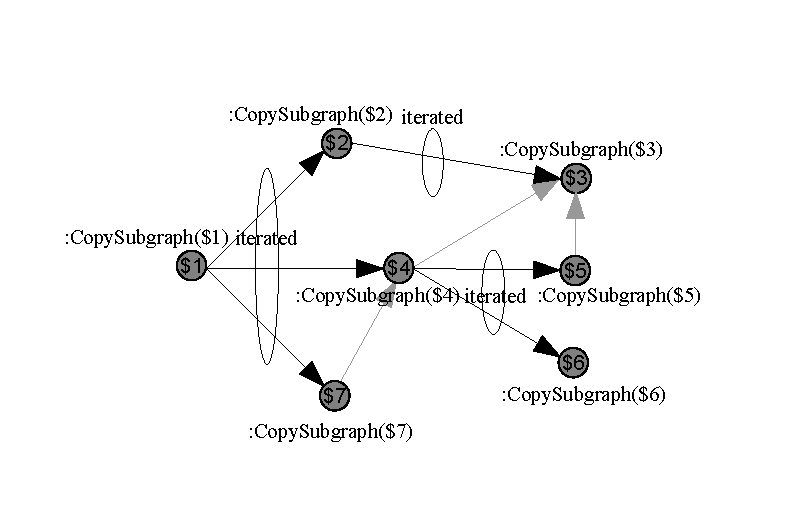
\includegraphics[width=\textwidth]{fig/SpanningTree}
  \caption{Matching a \indexed{spanning tree} in a graph}
  \label{figspanningtree}
\end{figure}

  \begin{example}\label{graphcompex}
    \begin{grgen}
pattern MatchSubgraph(root:Node, ref nodes:set<Node>)
{
  iterated { // match spanning tree of graph from root on
    root --> ch:Node;
    ms:MatchSubgraph(ch, nodes);

    modify {
      ms();
    }
  }

  modify {
    eval { nodes.add(root); } // build node set inducing graph
  }
}
    \end{grgen}
  \end{example}

The second step is to compute an induced subgraph from the node set collected, that can be done easily with the \texttt{inducedSubgraph} subgraph operation introduced in \ref{sec:subgraphop}:\\ \verb#exec sub:graph=inducedSubgraph(nodes)#.

The third step consists of comparing the subgraphs we filleted out of the common host graph with the graph comparison operators introduced in table \ref{compandgraph}:\\
\verb#exec if{sub1==sub2; doIso; doNonIso}#.

In case each such subgraph needs to be compared more than once it is recommended to add an attribute of type \texttt{graph} (see chapter \ref{cha:container}) to the subgraph starting anchor nodes, to assign the induced subgraph to this attribute, and to compare the subgraphs stored in these attribute.
This saves us the cost of computing the attributes and allows for further internal optimizations which 
may result in huge speedups.

\begin{warning}
The subgraph is not adapted automatically when the host graph changes, if this happens you must compute the stored subgraph anew manually.
\end{warning}

\noindent The comparison is then typically done with an idiom as such:\\
\verb#exec if{ for{other:AnchorNodeType; {curSub!=other.sub}} ; doNonIso(curSub)}# 
or such:\\
\verb#exec if{ for{other:graph in setOfCandidates; {curSub!=other}} ; doNonIso(curSub)}#.

Isomorphy comparison is an expensive operation, you can gain considerable speedups by using the parallelizable \texttt{equalsAny} function (cf. \ref{sec:subgraphop}) (and by specifying the number of worker threads (cf. \ref{sec:performanceparallel}), otherwise only a single one is used, saving you only the effort of manually coding the loop). 
In order to use this function you have to supply and maintain a set of the known subgraphs to check against in addition. 

\section{Copying Structures}\label{subsub:copystructure}\indexmain{subgraph copying}\indexmainsee{copy structure}{subgraph copying}
Structures are copied in two passes, the first consists of copying and collecting all nodes of interest, the second of copying all edges of interest in between the nodes.

The first pass consists of covering the nodes of the structure one wants to copy with iterated subpatterns,
in the same way as already introduced in \ref{subsub:comparestructure},
i.e. subpatterns which match from a root node on with iterateds along the incident edges into breadth,
employing a subpattern again on the node opposite to the root node to match into depth.
In the example we match the entire subgraph from a root node on, if one wants to copy a more constrained subgraph one can simple constrain the types, directions, and structures in the iterated subpattern covering the nodes.
The nodes are copied with the \texttt{copy} operators and a storagemap is filled, storing for every node copied its copy.

  \begin{example}
The example shows very generally how a subgraph reachable from a root node by incident edges can get copied, collecting and copying the nodes along a \indexed{spanning tree} from the root node on, then copying the edges in between the nodes in a second run afterwards. The edges get connected to the correct node copies via a mapping from the old to the new nodes remembered in a storage-map (\indexed{traceability} map).
    \begin{grgen}
pattern CopySubgraph(root:Node, ref oldToNew:map<Node, Node>)
{
  iterated { // match spanning tree of graph from root on
    root <--> ch:Node;
    cs:CopySubgraph(ch, oldToNew);

    modify {
      cs();
    }
  }

  modify {
    newroot:copy<root>; // copy nodes
    eval { oldToNew.add(root, newroot); }
    exec( [CopyOutgoingEdge(root, oldToNew)] ); // deferred copy edges
  }
}

rule CopyOutgoingEdge(n:Node, ref oldToNew:map<Node, Node>)
{
  n -e:Edge-> m:Node;
  hom(n,m); // reflexive edges
  nn:Node{oldToNew[n]}; nm:Node{oldToNew[m]};
  hom(nn,nm); // reflexive edges

  modify {
    nn -ee:copy<e>-> nm;
  }
}
    \end{grgen}
  \end{example}

The second pass is started after the structure matching ended by executing the deferred execs which were issued for every node handled.
Each \texttt{exec} copies all outgoing edges (one could process all incoming edges instead) of a node:
for each edge leaving the original node towards another original node a copy is created in between the copy of the original node and the copy of the other node.
The copies are looked up with the original nodes from the storage map (which fails for target nodes outside of the subgraph of interest).
Here too one could constrain the subgraph copied by filtering certain edges.
In case of undirected edges one would have to prevent that edges get copied twice (once for every incident node). This would require a visited flag for marking the already copied edges or a storage receiving them, queried in the edge copying pattern and set/filled in the edge copying rewrite part.

The example can be found in the \texttt{tests/copyStructure} directory.
Without storagemaps one would have to pollute the graph model with helper edges linking the original to the copied nodes.

\subsection{Built-In Graph Copying}\label{builtingraphcopying}
In contrast to the just introduced general copying of an entire graph, you may choose a limited form of copying subgraphs.
This is enabled by the \texttt{insertInduced} and \texttt{insertDefined} operations introduced in \ref{sec:subgraphop}, which add a clone of the subgraph induced by the set of nodes or set of edges given as first argument to the host graph.
The clone of the second argument node or edge which was inserted into the host graph is returned as anchor element for further operations.

Before you can apply these operations you must collect the nodes or edges which are used to compute the induced subgraph.
Besides building the sets element-by-element with \texttt{add}-methods you may use set returning functions, e.g. \texttt{adjacent} introduced in \ref{neighbouringelementsfunctions}, which returns the set of all the nodes adjacent to the node given as (first) argument.

Employing \texttt{insertInduced(adjacent())} is a common idiom for copying a subgraph when the host graph is partitioned into multiple subgraphs in the following way:
A special node type \texttt{Graph} and a special edge type \texttt{contains} are introduced into the graph model. 
Every subgraph is represented by a \texttt{Graph} anchor node.
From these anchor nodes on \texttt{contains} edges lead to all the non-subgraph nodes contained in the corresponding subgraph.
With this modelling, all nodes in a subgraph are easily reachable from one anchor node via \texttt{adjacent}, and the entire subgraph can be easily retrieved by using \texttt{inducedSubgraph} or copied by \texttt{insertInduced}.
Besides this simplified manipulation, the graph can be easily visualized as being partitioned into multiple subgraphs with a \texttt{dump add node Graph group by contains} graph visualization command (see \ref{sub:visual} for more on this).


\section{Data Flow Analysis for Computing Reachability}\label{subsub:flow}\indexmain{flow equations}\indexmain{data flow analysis}\indexmain{reachability}
%todo: refine this nightly hacked section
%add dominance computation

In compiler construction, given a program graph, one wants to compute non-local properties in order to transform the program graph.
This is normally handled within the framework of data flow analysis, which employs flow equations telling how property values of a node are influenced by property values of the predecessor or successor nodes in addition to the node's local share on the overall information, with the predecessor or successor nodes being again influenced by their predecessor or successor nodes.
Property values are modeled as sets; the information is propagated around the graph until a fix point is reached (the operations must be monotone in order for a fix point to exist on the finite domain of discourse).
You might be interested in the transparencies under \url{http://www2.imm.dtu.dk/~riis/PPA/slides2.pdf} for some reading on this topic;
especially as this is a general method to compute non-local informations over graphs not limited to compiler construction.

We'll apply a backward may analysis (with only $gen$ but no $kill$ information) to compute for each node the nodes which can be reached from this node.
Reachability is an interesting property if you have to do a lot of iterated path checks:
instead of computing the itererated path with a recursive pattern each and every time you must check for it,
compute it once and just look it up from then on.
If you need to check several paths which must be disjoint you won't get around employing recursive subpatterns with one locking the elements for the other; but even in this case the precomputed information should be valuable (unless the graph is heavily connected), constraining the search to source and target nodes between which a path does exist, eliminating nodes which are not connected.

The reachability information will be stored in a storage set per node of the graph (indeed, we trade memory space for execution speed):
  \begin{example}
    \begin{grgen}
node class N
{
	reachable:set<N>;
}
    \end{grgen}
  \end{example}

The analysis begins with initializing all the storage sets with the local information about the direct successors by employing the following rule on all possible matches:
  \begin{example}
    \begin{grgen}
rule directReachability
{
  hom(n,m);
  n:N --> m:N;

  modify {
    eval { n.reachable.add(m); }
  }
}
    \end{grgen}
  \end{example}

The analysis works by keeping a global todo-set \verb#todo# containing all the nodes which need to be (re-)visited,
because the information in one of their successors changed;
this set is initialized with all nodes available using the sequence \verb#[addAllNodesToWorkset(todo)]#).

From then on in each iteration step a node \verb#n# is removed with \verb#(n)=pickAndRemove(todo)#, until the todo-set becomes empty, signaling the termination of the analysis; the node is processed by determining its successors \verb#[successors(n, succs)]#, adding the reachability information available in each successor to \verb#n# controlled by the sequence\\
\verb#for{s in succs; (changed)=propagateBackwards(n,s,changed)}#.\\
If the information in \verb#n# changed due to this, the predecessors of the node are added to the workset via \verb#if{changed;[addPredecessors(n,todo)]}#.

  \begin{example}
This is the core rule of the dataflow analysis: the reachability information from the successor node \texttt{s} in its \texttt{reachable} storage attribute is added to the storage attribute of the node \texttt{n} of interest; if the storage set changes this is written to the returned variable.
    \begin{grgen}
rule propagateBackwards(n:N, s:N, var changed:boolean) : (boolean)
{
  modify {
    eval { n.reachable |= s.reachable |> changed; }
    return(changed);
  }
}
    \end{grgen}
  \end{example}

The example can be found in the \texttt{tests/dataFlowAnalysis} directory, just add \texttt{debug} before the \texttt{exec} (or \texttt{xgrs}) in \texttt{dataFlowAnalysisForReachability.grs} and watch it run.
A sample situation showing a propagation step is given in \ref{figdataflow}.
The subgraph at the top-left is already handled as you can see by the reachable set displayed in each node.

\begin{figure}[htbp]
  \centering
  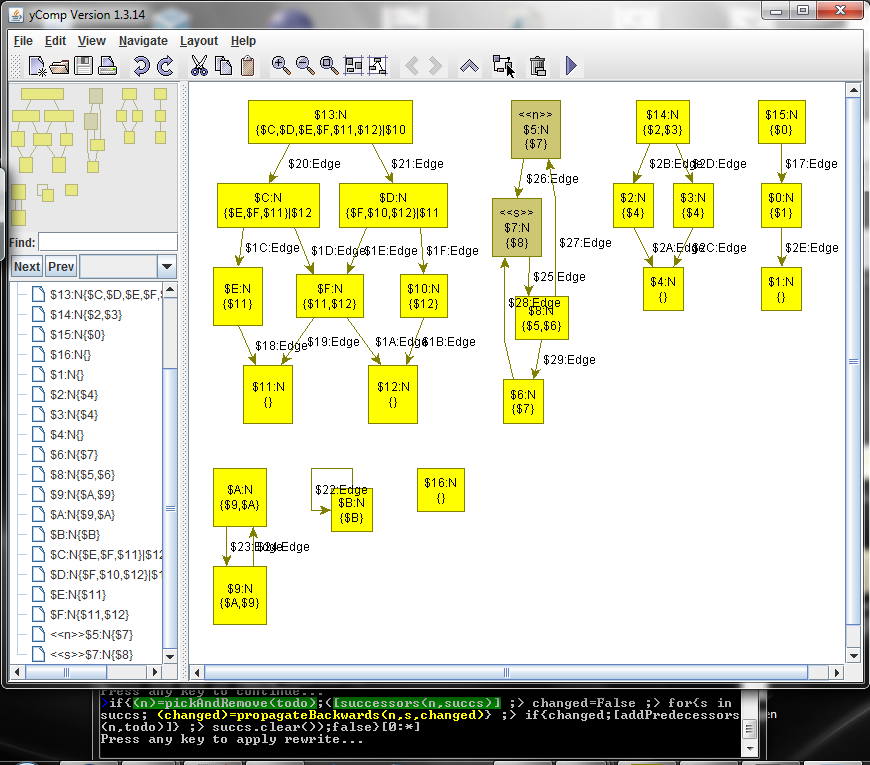
\includegraphics[width=\textwidth]{fig/Dataflow}
  \caption{Situation from dataflow analysis}
  \label{figdataflow}
\end{figure}

\subsubsection*{Worklist Based Data Flow Analysis}\indexmain{worklist}

The approach introduced above implements the basics but will not scale well to large graphs -- even medium sized graphs -- due to the random order the nodes are visited.
What is used in practice instead is a version employing a worklist built in postorder, so that a node is only visited after all its successor nodes have been processed.
For graphs without backedges, i.e. loops for program graphs, this gives an analysis which visits every node exactly once in the propagation phase.
For graphs with loops some nodes will be visited multiple times, but due to the ordering the analysis still terminates very fast.

The worklist is implemented directly in the graph by additional edges of the special type \verb#then# between the nodes, and a special node for the list start; the \verb#todo# set is kept, to allow for a fast "is the node already contained in the worklist"-check, used to save us from adding nodes again which are already contained (thus will be visited in the future anyway); i.e. the abstract worklist concept is implemented by the todo-set and the list added invasively to the graph.

  \begin{example}
    \begin{grgen}
edge class then; // for building worklist of nodes to be handled
    \end{grgen}
  \end{example}

\noindent The initial todo-set population of the simple approach is replaced by worklist constructing, successively advancing the last node of the worklist given by the \verb#last# variable; it starts with all nodes having no successor:\\
\verb#(last)=addFinalNodesToWorklist(last, todo)*#\\
Then iteratively all nodes which lead to them get added:\\
\verb#( (last)=addFurther(pos, last, todo)* ;> (pos)=switchToNextWorklistPosition(pos) )*#\\
In case of loops without terminal nodes we pick an arbitrary node from them:\\ \verb#(last)=addNotYetVisitedNodeToWorklist(last, todo)#\\
and add everything what leads to them, until every node was added to the worklist.

Now we can start the analysis, which works like the simple one does, utilizing the very same propagation rule,but follows the worklist instead of randomly picking from a todo-set, shrinking and growing the worklist along the way.

  \begin{example}
An example rule for worklist handling, adding a not yet contained node to the worklist; please note the quick check for containment via the set membership query.
    \begin{grgen}
rule addToWorklist(p:N, ref todo:set<N>, last:N) : (N)
{
  if{ !(p in todo); }

  modify {
    last -:then-> p;
    eval { todo.add(p); }
    return(p);
  }
}
    \end{grgen}
  \end{example}

  \begin{example}
An exmaple rule for worklist handling, removing the by-then processed node \texttt{pos} from the worklist.
    \begin{grgen}
rule nextWorklistPosition(pos:N, ref todo:set<N>) : (N)
{
  pos -t:then-> next:N;

  modify {
    delete(t);
    eval { todo.rem(pos); }
    return(next);
  }
}
    \end{grgen}
  \end{example}

The example can be found in the \texttt{tests/dataFlowAnalysis} directory, just add \texttt{debug} before the \texttt{exec} (or \texttt{xgrs}) in \texttt{dataFlowAnalysisForReachabilityWorklist.grs} and watch it run.
A sample situation showing a worklist building step is given in \ref{figworklist}.
The subgraph at the top-left is already handled as you can see by the reachable set displayed in each node.

\begin{figure}[htbp]
  \centering
  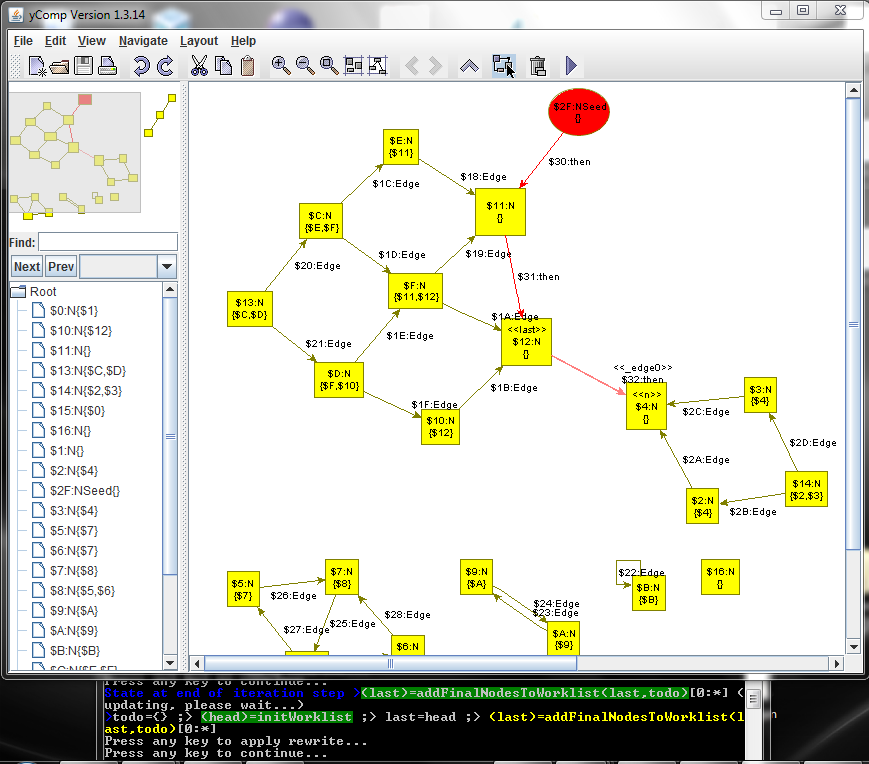
\includegraphics[width=\textwidth]{fig/Worklist}
  \caption{Situation from worklist building}
  \label{figworklist}
\end{figure}


\section{State Space Enumeration}\label{sec:statespaceenum}\indexmain{state space enumeration}
%todo: extend, refine this quick-hacked text

State space enumeration can be programmed in GrGen.NET utilizing the sequence constructs introduced up so far.
GrGen.NET always operates on one host graph, over one combined model, applying actions from one combined rule set --- so everything is always within reach.
That is by far the most simple approach to graph transformation, and for a tool which is not specially geared towards enumerating state spaces what makes most sense.
Thus state space enumeration (or transformation between different graphs/models) must be realized within the one host graph.
This can be achieved by virtually partitioning the host graph into smaller graphs or subgraphs, following a convention like this one:
There are nodes of type \texttt{Graph} which are representing a state of the statespace; each such representative is an anchor node for a subgraph.
The containment in the subgraph is denoted by a \texttt{contains} edge from a node of type \texttt{Graph} to all the nodes contained in this (sub)graph.
The edges between the \texttt{Graph} nodes give the relationship between the subgraphs, i.e. successorship between the states of the statespace.
The edges between the non-\texttt{Graph} nodes are the "normal" graph edges inside the subgraphs.

The key ingredients for state space enumeration then are
\begin{itemize}
	\item The aforementioned modelling with anchor nodes linking to the subgraphs, i.e. states
	\item Backtracking angles --- they allow to recursively enumerate and apply the matches of a rule found, exhaustively stepping through the state space, rolling back the effects on the graph of the previous match tried before carrying out the next step (see section \ref{sec:extctrl})
	\item Pause insertions --- they allow to write the interesting subgraphs found during state space search out into the host graph while effects recording of backtracking supervision is paused, so that they are not rolled back during backtracking (see section \ref{sec:extctrl})
	\item Recursive sequences --- they allow to nest backtracking angles dynamically, so it becomes possible to enumerate an entire state space with a sequence just implementing one backtracking step (see section \ref{sec:sequencedefinition})
	\item The capability to create a copy of a subgraph and insert it into the host graph (see section \ref{subsub:copystructure}, esp. subsection \ref{builtingraphcopying})
	\item The ability to compare subgraphs (see section \ref{subsub:comparestructure}).
Implemented in an optimized way with a subgraph attribute in the anchor nodes which contains a copy of the subgraph in the host graph, ready to be compared to the current graph, in order to decide whether that one should be inserted into the state space or purged for being an isomorphic copy of an already available instance. Potentially even further improved with an additional set of subgraphs, compared against with the parallelizable \texttt{equalsAny} function.
	\item Adjacency and induced functions to compute the subgraphs from the host graph following the \texttt{contains} edges from the anchor nodes (see section \ref{neighbouringelementsfunctions}, Connectedness Queries and section \ref{sec:subgraphop}, Subgraph Operations)
	\item The \texttt{auto} filters from \ref{sub:extflt} finally allow to optimize performance by filtering symmetric matches stemming from automorphic patterns. This is a lot more efficient than creating states which are for sure isomorphic and filtering them later on by comparison with all the other states.
\end{itemize}

The modelling given above allows to employ the ability of GrGen.NET/yComp to visualize nested graphs from a flat graph by interpreting node containment along edges of a special type (cf. \ref{sub:visual}), ballooning the anchor node up to a subgraph. 

An example implementation of this approach with a variant utilizing isomorphy checking and a variant without isomorphy checking can be found in the \texttt{tests/statespace} folder.
Feel free to drop in some \texttt{debug} prefixes before the \texttt{exec} (/\texttt{xgrs}) used to watch the assembling of the state space graph.
Another example implementation can be found in the \texttt{tests/statespaceChemistry} folder.
It shows how to enumerate all possible reaction results derivable from a set of start molecules according to some reaction rules.
The molecules are just accumulated in the host graph, it is taken care by storage sets that each step only processes the ones available at the start of the step.
At the end, each resulting molecule (i.e. connected component) is exported as a \texttt{.grsi} file.

